\chapter{CI / CD} \label{cicd}
\section{Was ist CI/CD}

Es handelt sich hier um Methode, bei der den Kunden regelmäßig Apps bereitgestellt und alle Phasen der Anwendungsentwicklung automatisiert werden. Die Hauptkonzepte von CI/CD sind Continuous Integration, Continuous Delivery und Continuous Deployment. CI/CD löst die Probleme, welche die Integration von neuem Code für DevOps-Teams verursachen kann.

Insbesondere sorgt CI/CD für eine kontinuierliche Automatisierung und Überwachung über den gesamten App-Lifecycle hinweg, von der Integrations- und Test- bis hin zur Bereitstellungs- und Implementierungsphase. Diese zusammenhängenden Praktiken werden oft als „CI/CD-Pipeline“ bezeichnet, und sie werden durch eine agile Zusammenarbeit der DevOps-Teams unterstützt.

Die Abkürzung CI/CD hat unterschiedliche Bedeutungen. „CI“ bedeutet Continuous Integration, also der Automatisierungsprozess für Entwickler. Bei einer erfolgreichen CI werden regelmäßig neue Codeänderungen für Apps entwickelt, geprüft und in einem gemeinsamen Repository zusammengeführt. Damit soll der Konflikt verhindert werden, den zu viele Branches einer App verursachen können, wenn sie zeitgleich entwickelt werden.

„CD“ bedeutet Continuous Delivery bzw. Continuous Deployment. Dass sind verwandte Konzepte, die zuweilen synonym verwendet werden. Obwohl es bei beiden Konzepten um die Automatisierung weiterer Phasen der Pipeline geht, werden die Begriffe manchmal unterschiedlich verwendet, um das Ausmaß der Automatisierung zu verdeutlichen.

Continuous Delivery bedeutet üblicherweise, dass App-Änderungen eines Entwicklers automatisch auf Bugs getestet und in ein Repository (wie GitHub oder eine Container-Registry) hochgeladen werden, von wo aus sie vom Operations-Team in einer Live-Produktivumgebung bereitgestellt werden können. Dieser Vorgang ist die Antwort auf Transparenz- und Kommunikationsprobleme zwischen Dev- und Business-Teams. Damit soll sichergestellt werden, dass neuer Code mit minimalem Aufwand implementiert werden kann.

Continuous Deployment (das andere „CD“) kann sich auf die automatische Freigabe von Entwickleränderungen vom Repository zur Produktivphase beziehen, wo sie direkt vom Kunden genutzt werden können. Dieser Vorgang soll der Überlastung von Operations-Teams bei manuellen Prozessen entgegenwirken, die die Anwendungsbereitstellung verlangsamen. Continuous Development baut die Vorteile der Continuous Delivery aus, indem auch noch die nächste Phase der Pipeline automatisiert wird.
\begin{figure}[h]
	\centerline{
		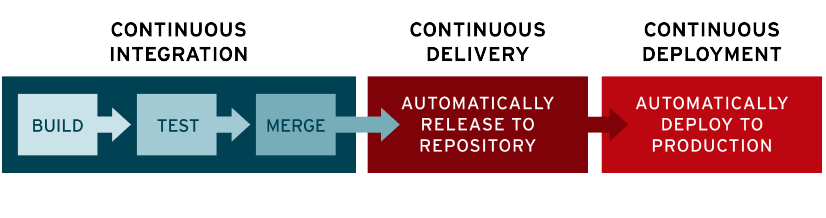
\includegraphics[width=0.8\textwidth]{./grafiken/ci-cd-flow-redhatsource.png}
	}
	\vskip0pt
	\caption{CI/CD Workflow} \label{fig:cicd}
\end{figure}

Manchmal sind mit CI/CD lediglich die zusammenhängenden Praktiken der Continuous Integration und der Continuous Delivery, manchmal aber auch alle drei Konzepte der Continuous Integration, Continuous Delivery und Continuous Deployment gemeint. Noch komplizierter wird das Ganze dadurch, dass mit Continuous Delivery zuweilen auch die Prozesse des Continuous Deployment mitgemeint sind.

Letztendlich bringen uns diese Details jedoch nicht weiter. Sehen Sie CI/CD einfach als Prozess an, der nicht selten als Pipeline visualisiert wird und der ein hohes Maß an kontinuierlicher Automatisierung und Überwachung bei der Anwendungsentwicklung umfasst. Je nach Fall hängt die Auslegung des Begriffs vom Grad der Automatisierung der CI/CD-Pipeline ab. Viele Unternehmen arbeiten zunächst mit CI und setzen den Prozess später mit der automatischen Bereitstellung und Implementierung fort, z. B. bei cloudnativen Apps.

\section{Continuous Integration}

Bei der modernen Anwendungsentwicklung arbeiten mehrere Entwickler an unterschiedlichen Features der gleichen App. Die gleichzeitige Zusammenführung aller Quellcode-Branches an einem Tag (auch bekannt als „Merge Day“) kann einen hohen Arbeits- und Zeitaufwand bedeuten. Der Grund dafür ist, dass Anwendungsänderungen von getrennt arbeitenden Entwicklern miteinander in Konflikt treten können, wenn sie zeitgleich durchgeführt werden. Dieses Problem kann sich verschlimmern, wenn jeder Entwickler seine eigene lokale Integrated Development Environment (IDE) definiert, statt im Team eine gemeinsame cloudbasierte IDE zu erstellen.

Mithilfe der Continuous Integration (CI) können Entwickler ihre Codeänderungen in einem gemeinsamen „Branch“ oder „Trunk“ der Anwendung viel häufiger zusammenführen, manchmal sogar täglich. Sobald die Änderungen eines Entwicklers zusammengeführt werden, werden sie in automatischen App-Builds und unterschiedlichen Stufen von Automatisierungsprüfungen (normalerweise Einheits- und Integrationstests) validiert. So wird sichergestellt, dass die Funktionsfähigkeit nicht beeinträchtigt wurde. Dabei müssen alle Klassen und Funktionen bis hin zu den verschiedenen Modulen der App getestet werden. Wenn die automatische Prüfung Konflikte zwischen aktuellem und neuem Code erkennt, lassen sich diese mithilfe von CI schneller und häufiger beheben.

\section{Continuous Delivery}

Nach der Automatisierung von Builds und Einheits- und Integrationstests bei der CI wird bei der Continuous Delivery auch die Freigabe des validierten Codes an ein Repository automatisch durchgeführt. Um also einen effizienten Continuous Delivery-Prozess zu gewährleisten, muss die CI bereits in Ihre Entwicklungs-Pipeline integriert sein. Ziel der Continuous Delivery ist eine Codebasis, die jederzeit in einer Produktivumgebung bereitgestellt werden kann.

Bei der Continuous Delivery umfasst jede Phase − von der Zusammenführung der Codeänderungen bis zur Bereitstellung produktionsreifer Builds − automatisierte Tests und Code-Freigaben. Am Ende dieses Prozesses kann das Operations-Team eine App schnell und einfach in der Produktivphase bereitstellen.

\section{Continuous Deployment}

Die abschließende Phase der CI/CD-Pipeline ist das Continuous Deployment. Als Erweiterung der Continuous Delivery, bei der produktionsreife Builds automatisch an ein Code-Repository freigegeben werden, wird beim Continuous Deployment auch die Freigabe einer App in die Produktivphase automatisiert. Da der Produktivphase in der Pipeline kein manuelles Gate vorgeschaltet ist, müssen beim Continuous Deployment die automatisierten Tests immer sehr gut durchdacht sein.

In der Praxis bedeutet Continuous Deployment, dass App-Änderungen eines Entwicklers binnen weniger Minuten nach ihrer Erstellung live gehen können (vorausgesetzt, sie bestehen den automatischen Test). Dies erleichtert eine kontinuierliche Integration von User Feedback ungemein. All diese zusammenhängenden CI/CD-Praktiken machen eine Anwendungsimplementierung weniger riskant, weil Änderungen in Teilen und nicht auf einmal freigegeben werden. Die Vorabinvestitionen sind allerdings beträchtlich, da automatische Tests für die diversen Prüf- und Release-Phasen in der CI/CD-Pipeline geschrieben werden müssen.\autocite{whatIsCICD}

\section{Gitlab Pipeline}

Pipelines sind top-level Komponenten der Continuous Integration, Delivery und Deployment. Pipelines umfassen:
\begin{itemize}
	\item Jobs, welche definieren \textit{was} auszuführen ist. Zum Beispiel gibt es Jobs, welche den Code kompilieren, Packete installieren und testen.
	\item Stages, welche definieren \textit{wann} Jobs auszuführen sind. Beispielsweise ist die Kompile-Stage üblicherweise vor der Test-Stage.
\end{itemize}

\autocite{gitlabPipelines}
